\chapter{Problem Analysis}
\todo{Delete the problem analysis but not the system requirements! Stef}
As discussed in chapter \ref{intro}, uneven module power generation due to mismatches may lead to inefficient overall power generation. If one of the modules of the PV array is generating below average, it will affect the overall power generation. This situation can be addressed by placing a bypass diode in parallel with every PV panel as shown in figure \ref{BYPASSED_MODULE}. This way the current can flow through the diode, maintaining a higher current in the string \cite{ArchitectureMIC}. However this solution will drive the power generation in the bypassed module to 0 and will cause a small power loss in the diode. Notice that the total power generated in the string is 120 W instead of 150 W. \todo{Why is it generating 120 W instead of 150 W? In the datasheet stands that the value 150 W is the starting voltage for the inverter TL}


\begin{figure}[H]
	\begin{center}
		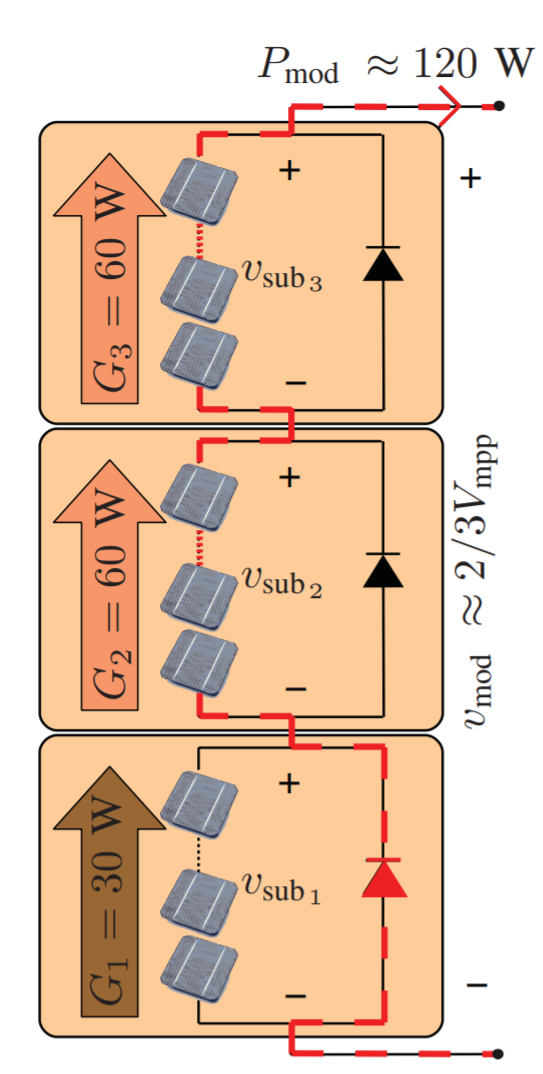
\includegraphics[width=0.25\textwidth]{../Pictures/Uneven_generation}
		\caption{PV module being bypassed by a diode\cite{ArchitectureMIC}.  %Architectures and Control of Submodule Integrated  DC–DC Converters for Photovoltaic Applications
		}
		\label{BYPASSED_MODULE}
	\end{center}	
\end{figure}

For avoiding the loss of the power generated by the bypassed PV module, a MIC may be used \cite{ArchitectureMIC}. %[Architectures and Control of Submodule Integrated  DC–DC Converters for Photovoltaic Applications] [Distributed Maximum Power Point Tracking in Photovoltaic Systems – Emerging Architectures and Control Methods] [Submodule Integrated Distributed Maximum Power Point Tracking for Solar Photovoltaic Applications] 
These MICs are usually micro-inverters or DC-DC converters which incorporate a MPPT algorithm in order to maximize the power generated by the module. 
Microinverters are composed of a DC-DC converter with MPPT and an inverter to convert the DC current from the PV directly to AC current to be connected to the grid. DC-DC converters need an inverter at their output if the desired load is the grid. 
As the micro-inverters have reported higher cost and slightly lower efficiency \cite{ArchitectureMIC} % [Submodule Integrated Distributed Maximum Power Point Tracking for Solar Photovoltaic Applications] 
the project will be focused in developing a DC-DC MIC for integrating it with a single PV panel.





